\documentclass[11pt]{article}
\usepackage{amsmath}
\usepackage{amssymb}
\usepackage{graphicx}
\usepackage{tabularx}
\usepackage{fancyhdr}
\usepackage{lastpage}

% Page layout
\usepackage[top=1in, bottom=1in, left=1in, right=1in]{geometry}

% Header and footer
\pagestyle{fancy}
\fancyhf{}
\rfoot{Page \thepage}
\renewcommand{\headrulewidth}{0pt}

% Modified Question command with left-aligned number
\newcommand{\questiona}[2]{
    \noindent\textbf{Q#2.} #1 \hfill \textbf{[1 Mark]}
}

\newcommand{\questionb}[2]{
    \noindent\textbf{Q#2.} #1 \hfill \textbf{[2 Marks]}
}

\begin{document}

% Title section with horizontal line
\begin{center}
    \Large\textbf{GATE 2017 - Computer Science (CS)} \\
    \large\textbf{General Aptitude and Technical Questions} \\
    \rule{\textwidth}{0.5pt} % Horizontal line below heading
\end{center}

\vspace{0.5cm}

\section*{General Aptitude}

\questiona{After Rajendra Chola returned from his voyage to Indonesia, he \_\_\_\_\_ to visit the temple in Thanjavur.}{1}
\begin{enumerate}
    \item[(A)] was wishing  
    \item[(B)] is wishing  
    \item[(C)] wished  
    \item[(D)] had wished  
\end{enumerate}
\vspace{0.5cm}

\questiona{Research in the workplace reveals that people work for many reasons \_\_\_\_\_.}{2}
\begin{enumerate}
    \item[(A)] money beside  
    \item[(B)] beside money  
    \item[(C)] money besides  
    \item[(D)] besides money  
\end{enumerate}
\vspace{0.5cm}

\questiona{Rahul, Murali, Srinivas and Arul are seated around a square table. Rahul is sitting to the left of Murali. Srinivas is sitting to the right of Arul. Which of the following pairs are seated opposite each other?}{3}
\begin{enumerate}
    \item[(A)] Rahul and Murali  
    \item[(B)] Srinivas and Arul  
    \item[(C)] Srinivas and Murali  
    \item[(D)] Srinivas and Rahul  
\end{enumerate}
\vspace{0.5cm}

\questiona{Find the smallest number \( y \) such that \( y \times 162 \) is a perfect cube.}{4}
\begin{enumerate}
    \item[(A)] 24  
    \item[(B)] 27  
    \item[(C)] 32  
    \item[(D)] 36  
\end{enumerate}
\vspace{0.5cm}

\questiona{The probability that a 4-digit number does NOT contain the digits 0, 5, or 9 is}{5}
\begin{enumerate}
    \item[(A)] 0.3\%  
    \item[(B)] 0.6\%  
    \item[(C)] 0.7\%  
    \item[(D)] 0.9\%  
\end{enumerate}
\vspace{0.5cm}

\questionb{“The hold of the nationalist imagination on our colonial past is such that anything inadequately or improperly nationalist is just not history.” Which of the following statements best reflects the author’s opinion?}{6}
\begin{enumerate}
    \item[(A)] Nationalists are highly imaginative.  
    \item[(B)] History is viewed through the filter of nationalism.  
    \item[(C)] Our colonial past never happened.  
    \item[(D)] Nationalism has to be both adequately and properly imagined.  
\end{enumerate}
\vspace{0.5cm}

\questionb{Six people are seated around a circular table. There are at least two men and two women. There are at least three right-handed persons. Every woman has a left-handed person to her immediate right. None of the women are right-handed. The number of women at the table is}{7}
\begin{enumerate}
    \item[(A)] 2  
    \item[(B)] 3  
    \item[(C)] 4  
    \item[(D)] Cannot be determined  
\end{enumerate}
\vspace{0.5cm}

\questionb{The expression \( (\lvert x + y \rvert - \lvert x - y \rvert)/2 \) is equal to}{8}
\begin{enumerate}
    \item[(A)] the maximum of \( x \) and \( y \)  
    \item[(B)] the minimum of \( x \) and \( y \)  
    \item[(C)] \( 1 \)  
    \item[(D)] none of the above  
\end{enumerate}
\vspace{0.5cm}

\questionb{Arun, Gulab, Neel and Shweta must choose one shirt each from a pile of four shirts coloured red, pink, blue and white respectively. Arun dislikes the colour red and Shweta dislikes the colour white. Gulab and Neel like all the colours. In how many different ways can they choose the shirts so that no one has a shirt with a colour he or she dislikes?}{9}
\begin{enumerate}
    \item[(A)] 21  
    \item[(B)] 18  
    \item[(C)] 16  
    \item[(D)] 14  
\end{enumerate}
\vspace{0.5cm}

\questionb{A contour line joins locations having the same height above the mean sea level. The following is a contour plot of a geographical region. Contour lines are shown at 25 m intervals in this plot. If in a flood, the water level rises to 525 m, which of the villages P, Q, R, S, T get submerged?}{10}
\begin{center}
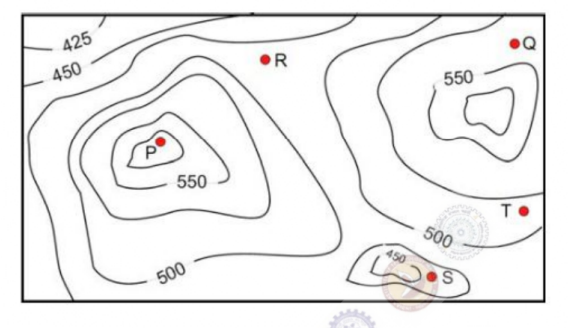
\includegraphics[width=0.5\textwidth]{figures/10.png}
\end{center}
\begin{enumerate}
    \item[(A)] P, Q  
    \item[(B)] P, Q, T  
    \item[(C)] R, S, T  
    \item[(D)] Q, R, S  
\end{enumerate}
\vspace{0.5cm}

\section*{Technical Section}

\questiona{The statement \( (\neg p) = (\neg q)\) is logically equivalent to which of the statements below?}{1}
\begin{center}
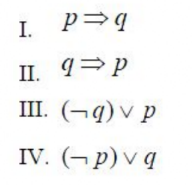
\includegraphics[width=0.3\textwidth]{figures/1.png}
\end{center}
\begin{enumerate}
    \item[(A)] I only  
    \item[(B)] I and IV only  
    \item[(C)] I only  
    \item[(D)] II and III only  
\end{enumerate}
\vspace{0.5cm}

\questiona{Consider the first-order logic sentence \( F: \forall x (\exists y\, R(x,y)) \). Assuming non-empty logical domains, which of the sentences below are implied by \( F \)?}{2}
\begin{center}
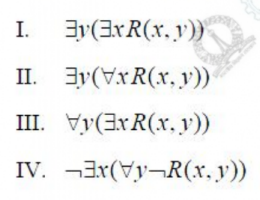
\includegraphics[width=0.25\textwidth]{figures/2.png}
\end{center}
\begin{enumerate}
    \item[(A)] IV only  
    \item[(B)] I and IV only  
    \item[(C)] II only  
    \item[(D)] II and III only  
\end{enumerate}
\vspace{0.5cm}

\questiona{Let \( c_1, \ldots, c_n \) be scalars, not all zero, such that \( \sum_{i=1}^{n} c_i a_i = 0 \) where \( a_i \) are column vectors in \( \mathbb{R}^n \). Consider the set of linear equations \( Ax = b \) where \( A = [a_1, \ldots, a_n] \) and \( b = \sum_{i=1}^{n} a_i \). The set of equations has}{3}
\begin{enumerate}
    \item[(A)] a unique solution at \( x = J_n \), where \( J_n \) denotes an \( n \)-dimensional vector of all 1  
    \item[(B)] no solution  
    \item[(C)] infinitely many solutions  
    \item[(D)] finitely many solutions  
\end{enumerate}
\vspace{0.5cm}

\questiona{Consider the following functions from positive integers to real numbers:  
100, 10, \( \sqrt{n} \), \( \log n \), \( n \).  
The CORRECT arrangement of the above functions in increasing order of asymptotic complexity is:}{4}
\begin{enumerate}
    \item[(A)] \( \log n, \sqrt{n}, 10, n, 100 \)  
    \item[(B)] \( 10, \log n, \sqrt{n}, n, 100 \)  
    \item[(C)] \( 10, \sqrt{n}, \log n, n, 100 \)  
    \item[(D)] \( \log n, 10, \sqrt{n}, n, 100 \)  
\end{enumerate}
\vspace{0.5cm}

\questiona{Consider the following table:  
\begin{center}
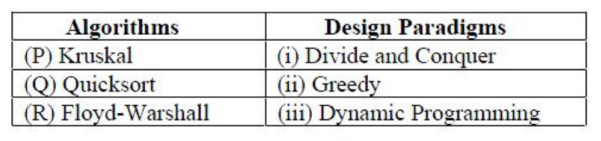
\includegraphics[width=0.5\textwidth]{figures/5.png}
\end{center}
Match the algorithms to the design paradigms they are based on.}{5}
\begin{enumerate}
    \item[(A)] P \(\rightarrow\) (ii), Q \(\rightarrow\) (i), R \(\rightarrow\) (iii)  
    \item[(B)] P \(\rightarrow\) (iii), Q \(\rightarrow\) (i), R \(\rightarrow\) (ii)  
    \item[(C)] P \(\rightarrow\) (i), Q \(\rightarrow\) (iii), R \(\rightarrow\) (ii)  
    \item[(D)] P \(\rightarrow\) (ii), Q \(\rightarrow\) (iii), R \(\rightarrow\) (i)  
\end{enumerate}
\vspace{0.5cm}

\questiona{Let \( T \) be a binary search tree with 15 nodes. The minimum and maximum possible heights of \( T \) are:  
(Note: The height of a tree with a single node is 0.)}{6}
\begin{enumerate}
    \item[(A)] 4 and 15 respectively  
    \item[(B)] 3 and 14 respectively  
    \item[(C)] 4 and 14 respectively  
    \item[(D)] 3 and 15 respectively  
\end{enumerate}
\vspace{0.5cm}

\questiona{The \( n \)-bit fixed-point representation of an unsigned real number \( X \) uses \( f \) bits for the fraction part. Let \( i = n - f \). The range of decimal values for \( X \) in this representation is:}{7}
\begin{enumerate}
    \item[(A)] \( 2^i \) to \( 2^f \)  
    \item[(B)] \( 2^i \) to \( (2 - 2^{-f}) \)  
    \item[(C)] \( 0 \) to \( 2^i \)  
    \item[(D)] \( 0 \) to \( (2^i - 2^{-f}) \)  
\end{enumerate}
\vspace{0.5cm}

\questiona{Consider the C code fragment given below.}{8}
\begin{center}
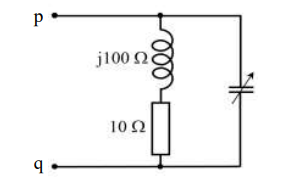
\includegraphics[width=0.5\textwidth]{figures/8.png}
\end{center}
Assuming that \( m \) and \( n \) point to valid NULL-terminated linked lists, invocation of `join` will
\begin{enumerate}
    \item[(A)] append list \( m \) to the end of list \( n \) for all inputs.  
    \item[(B)] either cause a null pointer dereference or append list \( m \) to the end of list \( n \).  
    \item[(C)] cause a null pointer dereference for all inputs.  
    \item[(D)] append list \( n \) to the end of list \( m \) for all inputs.  
\end{enumerate}
\vspace{0.5cm}

\questiona{When two 8-bit numbers \( A_7...A_0 \) and \( B_7...B_0 \) in 2’s complement representation (with \( A_0 \) and \( B_0 \) as the least significant bits) are added using a ripple-carry adder, the sum bits obtained are \( S_7...S_0 \) and the carry bits are \( C_1...C_8 \). An overflow is said to have occurred if:}{9}
\begin{enumerate}
    \item[(A)] the carry bit \( C_8 \) is 1  
    \item[(B)] all the carry bits \( C_1...C_8 \) are 1  
    \item[(C)] \( (A_7 + B_7 - S_7 + A_6 + B_6 - S_6) \) is 1  
    \item[(D)] \( (A_7 \land B_7 \land \neg S_7) \lor (\neg A_7 \land \neg B_7 \land S_7) \) is 1  
\end{enumerate}
\vspace{0.5cm}

\questiona{Consider the following context-free grammar over the alphabet \( \Sigma = \{a, b, c\} \) with \( S \) as the start symbol:  
\( S \rightarrow abScT \,|\, abcT \)  
\( T \rightarrow bT \,|\, b \)  
Which one of the following represents the language generated by the above grammar?}{10}
\begin{enumerate}
    \item[(A)] \( \{(ab)^n(cb)^m \mid n = 1\} \)  
    \item[(B)] \( \{(ab)^n cb^{m_1} cb^{m_2} \ldots cb^{m_n} \mid n, m_1, m_2, \ldots, m_n \geq 1\} \)  
    \item[(C)] \( \{(ab)^n cb^m \mid m, n \geq 1\} \)  
    \item[(D)] \( \{(ab)^n (cb)^m \mid m, n \geq 1\} \)  
\end{enumerate}
\vspace{0.5cm}

\questiona{Consider the C struct defined below:  
\begin{center}
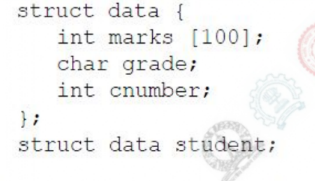
\includegraphics[width=0.5\textwidth]{figures/11.png}
\end{center}
The base address of \texttt{student} is available in register \texttt{R1}. The field \texttt{student.grade} can be accessed efficiently using}{11}
\begin{enumerate}
    \item[(A)] Post-increment addressing mode, \texttt{(R1)+}  
    \item[(B)] Pre-decrement addressing mode, \texttt{--(R1)}  
    \item[(C)] Register direct addressing mode, \texttt{R1}  
    \item[(D)] Index addressing mode, \texttt{X(R1)}, where \texttt{X} is an offset represented in 2’s complement 16-bit representation  
\end{enumerate}
\vspace{0.5cm}

\questiona{Consider the following intermediate program in three-address code:}{12}
\begin{center}
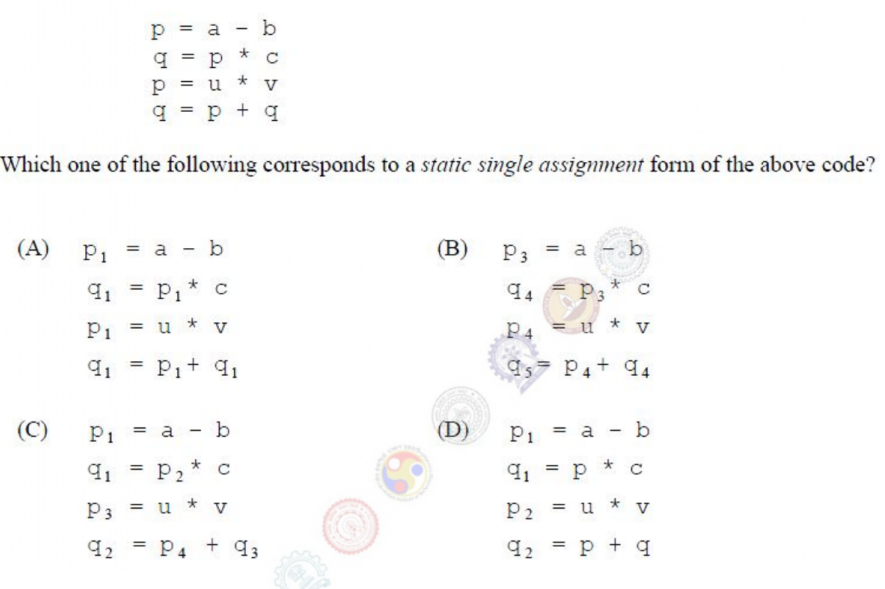
\includegraphics[width=1\textwidth]{figures/12.png}
\end{center}
\vspace{0.5cm}

\questiona{Consider the following C code:}{13}
\begin{center}
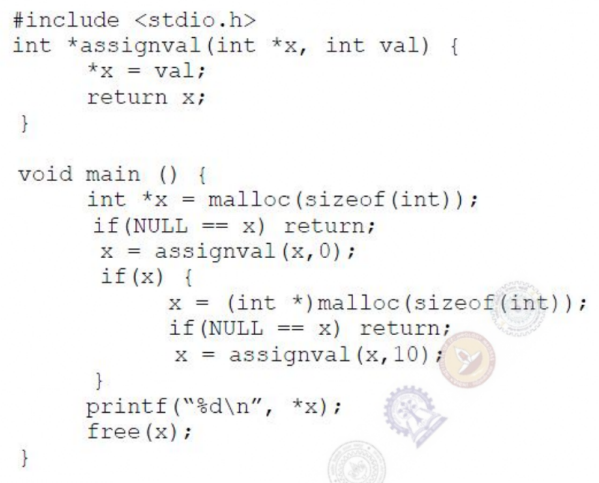
\includegraphics[width=0.5\textwidth]{figures/13.png}
\end{center}
The code suffers from which one of the following problems?  
\begin{enumerate}
    \item[(A)] compiler error as the return of \texttt{malloc} is not typecast appropriately  
    \item[(B)] compiler error because the comparison should be made as \texttt{x == NULL} and not as shown  
    \item[(C)] compiles successfully but execution may result in dangling pointer  
    \item[(D)] compiles successfully but execution may result in memory leak  
\end{enumerate}
\vspace{0.5cm}

\questiona{A TCP client and a TCP server are running on two different machines. After completing data transfer, the TCP client calls \texttt{close} to terminate the connection and a FIN segment is sent to the TCP server. Server-side TCP responds by sending an ACK, which is received by the client-side TCP. As per the TCP connection state diagram (RFC 793), in which state does the client-side TCP connection wait for the FIN from the server-side TCP?}{14}
\begin{enumerate}
    \item[(A)] LAST-ACK  
    \item[(B)] TIME-WAIT  
    \item[(C)] FIN-WAIT-1  
    \item[(D)] FIN-WAIT-2  
\end{enumerate}
\vspace{0.5cm}

\questiona{A sender \( S \) sends a message \( m \) to receiver \( R \), which is digitally signed by \( S \) with its private key. In this scenario, one or more of the following security violations can take place.  
(I) \( S \) can launch a birthday attack to replace \( m \) with a fraudulent message.  
(II) A third-party attacker can launch a birthday attack to replace \( m \) with a fraudulent message.  
(III) \( R \) can launch a birthday attack to replace \( m \) with a fraudulent message.  
Which of the following are possible security violations?}{15}
\begin{enumerate}
    \item[(A)] (I) and (II) only  
    \item[(B)] (II) only  
    \item[(C)] (III) only  
    \item[(D)] (II) and (III) only  
\end{enumerate}
\vspace{0.5cm}

\questiona{The following functional dependencies hold true for the relational schema \( R(V, W, X, Y, Z) \):  
\[
\begin{aligned}
& V \rightarrow W \\
& VW \rightarrow X \\
& Y \rightarrow VX \\
& Y \rightarrow Z \\
\end{aligned}
\]
Which of the following is an irreducible equivalent for this set of functional dependencies?}{16}
\begin{enumerate}
    \item[(A)] \( V \rightarrow W, V \rightarrow X, Y \rightarrow V, Y \rightarrow Z \)  
    \item[(B)] \( V \rightarrow W, VW \rightarrow X, Y \rightarrow V, Y \rightarrow Z \)  
    \item[(C)] \( V \rightarrow W, W \rightarrow X, Y \rightarrow V, Y \rightarrow X \)  
    \item[(D)] \( V \rightarrow W, VW \rightarrow X, Y \rightarrow V, Y \rightarrow X \)  
\end{enumerate}
\vspace{0.5cm}

\questiona{Consider the following grammar:  
\[
\begin{aligned}
P &\rightarrow xQRS \\
Q &\rightarrow z \\
R &\rightarrow w \,|\, \epsilon\\
S &\rightarrow y
\end{aligned}
\]
What is FOLLOW(Q)?}{17}
\begin{enumerate}
    \item[(A)] \{R\}  
    \item[(B)] \{w\}  
    \item[(C)] \{w, v\}  
    \item[(D)] \{w, \$\}  
\end{enumerate}
\vspace{0.5cm}

\questiona{Threads of a process share}{18}
\begin{enumerate}
    \item[(A)] global variables but not heap  
    \item[(B)] heap but not global variables  
    \item[(C)] neither global variables nor heap  
    \item[(D)] both heap and global variables  
\end{enumerate}
\vspace{0.5cm}

\questiona{Let \( X \) be a Gaussian random variable with mean 0 and variance \( \sigma^2 \). Let \( Y = \max(X, 0) \) where \( \max(a, b) \) is the maximum of \( a \) and \( b \). The median of \( Y \) is}{19}

\vspace{0.5cm}

\questiona{Let \( T \) be a tree with 10 vertices. The sum of the degrees of all the vertices in \( T \) is}{20}

\vspace{0.5cm}

\questiona{Consider the Karnaugh map given below, where X represents “don’t care” and blank represents 0.  
Assume for all inputs \( (a, b, c, d) \), the respective complements \( (\overline{a}, \overline{b}, \overline{c}, \overline{d}) \) are also available.  
The above logic is implemented using 2-input NOR gates only. The minimum number of gates required is:}{21}
\begin{center}
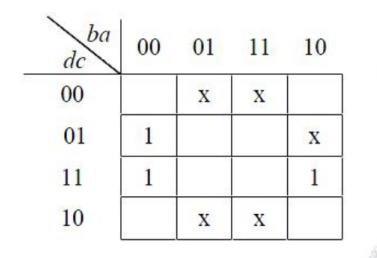
\includegraphics[width=0.5\textwidth]{figures/21.png}
\end{center}

\vspace{0.5cm}

\questiona{Consider the language \( L \) given by the regular expression \( (a + b)^* b (a + b) \) over the alphabet \( \{a, b\} \).  
The smallest number of states needed in a deterministic finite-state automaton (DFA) accepting \( L \) is:}{22}

\vspace{0.5cm}

\questiona{Consider a database that has the relation schema \texttt{EMP}(\texttt{EmpId}, \texttt{EmpName}, \texttt{DeptName}).  
An instance of the schema and a SQL query on it are given below.}{23}
\begin{center}
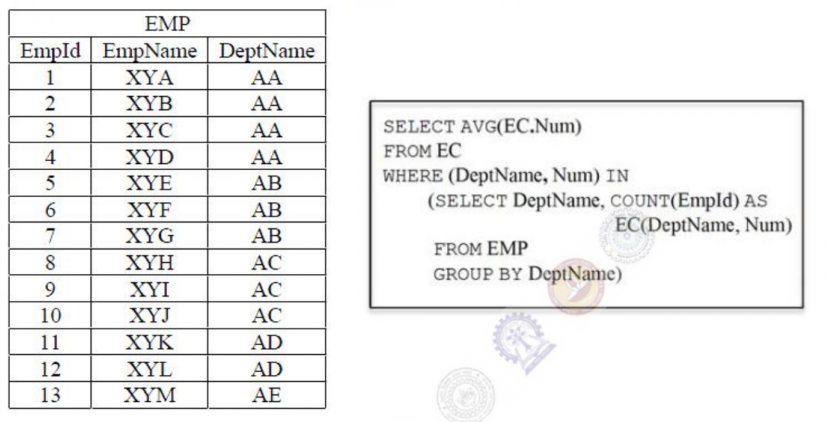
\includegraphics[width=0.9\textwidth]{figures/23.png}
\end{center}
The output of executing the SQL query is:

\vspace{0.5cm}

\questiona{Consider the following CPU processes with arrival times (in milliseconds) and length of CPU bursts (in milliseconds) as given below:  
\begin{center}
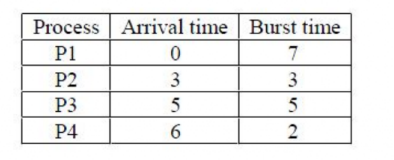
\includegraphics[width=0.5\textwidth]{figures/24.png}
\end{center}
If the pre-emptive shortest remaining time first scheduling algorithm is used to schedule the processes, then the average waiting time across all processes is \_\_\_\_ milliseconds.}{24}
\vspace{0.5cm}

\questiona{Consider a two-level cache hierarchy with L1 and L2 caches.  
An application incurs 1.4 memory accesses per instruction on average. For this application, the miss rate of L1 cache is 0.1;  
the L2 cache experiences, on average, 7 misses per 1000 instructions. The miss rate of L2 expressed correct to two decimal places is:}{25}
\vspace{0.5cm}

\questionb{Let \( G = (V, E) \) be any connected undirected edge-weighted graph. The weights of the edges in \( E \) are positive and distinct.  
Consider the following statements:  
(I) Minimum Spanning Tree of \( G \) is always unique.  
(II) Shortest path between any two vertices of \( G \) is always unique.  
Which of the above statements is/are necessarily true?}{26}
\begin{enumerate}
    \item[(A)] (I) only  
    \item[(B)] (II) only  
    \item[(C)] Both (I) and (II)  
    \item[(D)] Neither (I) nor (II)  
\end{enumerate}
\vspace{0.5cm}

\questionb{A multithreaded program \( P \) executes with \( v \) number of threads and uses \( x \) number of locks for ensuring mutual exclusion while operating on shared memory locations.  
All locks in the program are non-reentrant, i.e., if a thread holds a lock \( l \), then it cannot re-acquire lock \( l \) without releasing it.  
If a thread is unable to acquire a lock, it blocks until the lock becomes available.  
The minimum value of \( x \) and the minimum value of \( v \) together for which execution of \( P \) can result in a deadlock are \_\_\_\_\_.}{27}
\begin{center}
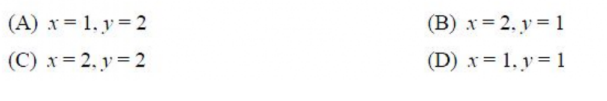
\includegraphics[width=0.8\textwidth]{figures/27.png}
\end{center}
\vspace{0.5cm}

\questionb{The value of \( \lim_{x \to 0} \frac{\sin(7x)}{-3x^5 + 2} \) is \_\_\_\_\_.}{28}
\vspace{0.5cm}

\questionb{Let \( p, q, r \) be propositions and the expression \( (p \rightarrow q) \rightarrow \neg r \) be a contradiction.  
Then, the expression \( (r \rightarrow p) \rightarrow q \) is}{29}
\begin{enumerate}
    \item[(A)] a tautology  
    \item[(B)] a contradiction  
    \item[(C)] always TRUE when \( p \) is FALSE  
    \item[(D)] always TRUE when \( q \) is TRUE  
\end{enumerate}
\vspace{0.5cm}

\questionb{Let \( u \) and \( v \) be two vectors in \( \mathbb{R}^n \) whose Euclidean norms satisfy \( \|u\| = 2\|v\| \).  
What is the value of \( \alpha \) such that \( w = u + \alpha v \) bisects the angle between \( u \) and \( v \)?}{30}
\begin{enumerate}
    \item[(A)] 2  
    \item[(B)] 1/2  
    \item[(C)] 1  
    \item[(D)] -1/2  
\end{enumerate}
\vspace{0.5cm}

\questionb{Let \( A \) be an \( n \times n \) real-valued square symmetric matrix of rank 2 with  
\[
\sum_{i=1}^{n} \sum_{j=1}^{n} A_{ij} = 50.
\]  
Consider the following statements about the eigenvalues of \( A \):  
(I) One eigenvalue must be in \( [-5, 5] \)  
(II) The eigenvalue with the largest magnitude must be strictly greater than 5  
Which of the above statements is/are necessarily CORRECT?}{31}
\begin{enumerate}
    \item[(A)] Both (I) and (II)  
    \item[(B)] (II) only  
    \item[(C)] (I) only  
    \item[(D)] Neither (I) nor (II)  
\end{enumerate}
\vspace{0.5cm}

\questionb{A computer network uses polynomials over GF(2) for error checking with 8 bits as information bits and uses \( x^3 + x + 1 \) as the generator polynomial to generate the check bits.  
In this network, the message 01011011 is transmitted as \_\_\_\_\_.}{32}
\vspace{0.5cm}

\questionb{Consider a combination of T and D flip-flops connected as shown below.}{33}
\begin{center}
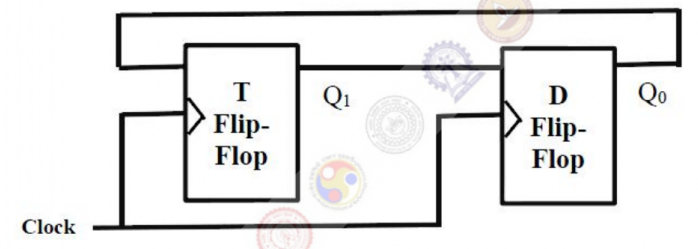
\includegraphics[width=0.5\textwidth]{figures/33.png}
\end{center}
Initially, both \( Q_0 \) and \( Q_1 \) are set to 1 (before the 1st clock cycle). The outputs
\begin{enumerate}
    \item[(A)] \( Q_1 Q_0 \) after the 3rd cycle are 11 and after the 4th cycle are 00 respectively  
    \item[(B)] \( Q_1 Q_0 \) after the 3rd cycle are 11 and after the 4th cycle are 01 respectively  
    \item[(C)] \( Q_1 Q_0 \) after the 3rd cycle are 00 and after the 4th cycle are 11 respectively  
    \item[(D)] \( Q_1 Q_0 \) after the 3rd cycle are 01 and after the 4th cycle are 01 respectively  
\end{enumerate}
\vspace{0.5cm}

\questionb{If \( G \) is a grammar with productions  
\[
S \rightarrow SaS \mid aSb \mid bSa \mid SS \mid \epsilon
\]  
where \( S \) is the start variable, then which one of the following strings is not generated by \( G \)?}{34}
\begin{enumerate}
    \item[(A)] abab  
    \item[(B)] aaab  
    \item[(C)] abbaa  
    \item[(D)] babba  
\end{enumerate}
\vspace{0.5cm}

\questionb{Consider the following two functions.}{35}
\begin{center}
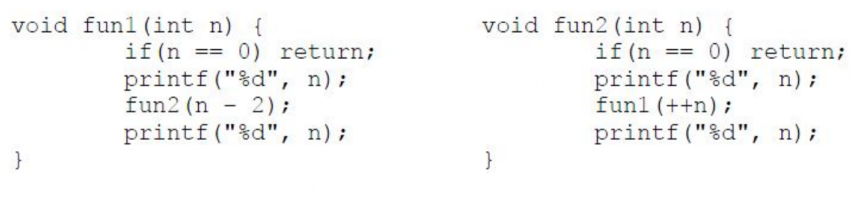
\includegraphics[width=0.8\textwidth]{figures/35.png}
\end{center}
The output printed when \texttt{fun1(5)} is called is:
\begin{enumerate}
    \item[(A)] 53423122233445  
    \item[(B)] 53423120112233  
    \item[(C)] 53423122132435  
    \item[(D)] 53423120213243  
\end{enumerate}
\vspace{0.5cm}

\questionb{Consider the C functions \texttt{foo} and \texttt{bar} given below.}{36}
\begin{center}
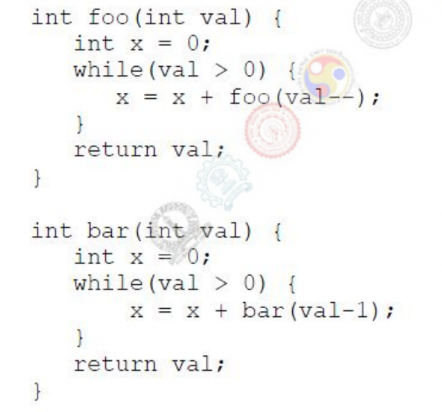
\includegraphics[width=0.5\textwidth]{figures/36.png}
\end{center}
Invocations of \texttt{foo(3)} and \texttt{bar(3)} will result in:
\begin{enumerate}
    \item[(A)] Return of 6 and 6 respectively  
    \item[(B)] Infinite loop and abnormal termination respectively  
    \item[(C)] Abnormal termination and infinite loop respectively  
    \item[(D)] Both terminating abnormally  
\end{enumerate}
\vspace{0.5cm}

\questionb{Consider the context-free grammars over the alphabet \( \{a, b, c\} \) given below.  
\( G_1: S \rightarrow aS b \mid T, \quad T \rightarrow cT \mid \epsilon \)  
\( G_2: S \rightarrow bS a \mid T, \quad T \rightarrow cT \mid \epsilon \)  
The language \( L(G_1) \cap L(G_2) \) is}{37}
\begin{enumerate}
    \item[(A)] Finite  
    \item[(B)] Not finite but regular  
    \item[(C)] Context-free but not regular  
    \item[(D)] Recursive but not context-free  
\end{enumerate}
\vspace{0.5cm}

\questionb{Consider the following languages over the alphabet \( \Sigma = \{a, b, c\} \):  
Let \( L_1 = \{a^m b^n c^m \mid m, n \geq 0\} \) and \( L_2 = \{a^m b^n c^n \mid m, n \geq 0\} \).  
Which of the following are context-free languages?  
(I) \( L_1 \cup L_2 \)  
(II) \( L_1 \cap L_2 \) }{38}
\begin{enumerate}
    \item[(A)] I only  
    \item[(B)] II only  
    \item[(C)] I and II  
    \item[(D)] Neither I nor II  
\end{enumerate}
\vspace{0.5cm}

\questionb{Let \( A \) and \( B \) be finite alphabets and let \( \# \) be a symbol outside both \( A \) and \( B \).  
Let \( f \) be a total function from \( A^* \) to \( B^* \). We say \( f \) is computable if there exists a Turing machine \( M \)  
which given an input \( x \in A^* \) always halts with \( f(x) \) on its tape. Let  
\[
L_f = \{x \# f(x) \mid x \in A^* \}
\]  
Which of the following statements is true:}{39}
\begin{enumerate}
    \item[(A)] \( f \) is computable if and only if \( L_f \) is recursive  
    \item[(B)] \( f \) is computable if and only if \( L_f \) is recursively enumerable  
    \item[(C)] If \( f \) is computable then \( L_f \) is recursive, but not conversely  
    \item[(D)] If \( f \) is computable then \( L_f \) is recursively enumerable, but not conversely  
\end{enumerate}
\vspace{0.5cm}

\questionb{Recall that Belady’s anomaly is that the page-fault rate may increase as the number of allocated frames increases.  
Now consider the following statements:  
S1: Random page replacement algorithm (where a page chosen at random is replaced) suffers from Belady’s anomaly  
S2: LRU page replacement algorithm suffers from Belady’s anomaly  
Which of the following is CORRECT?}{40}
\begin{enumerate}
    \item[(A)] S1 is true, S2 is true  
    \item[(B)] S1 is true, S2 is false  
    \item[(C)] S1 is false, S2 is true  
    \item[(D)] S1 is false, S2 is false  
\end{enumerate}
\vspace{0.5cm}

\questionb{Consider a database that has the relation schemas \texttt{EMP(EmpId, EmpName, DeptId)} and  
\texttt{DEPT(DeptName, DeptId)}. Note that the \texttt{DeptId} can be permitted to be NULL in the relation \texttt{EMP}.  
Consider the following queries on the database expressed in tuple relational calculus:  
\\ (I) \( \{t \mid \exists u \in EMP (t[\text{EmpName}] = u[\text{EmpName}] \land \exists v \in DEPT (t[\text{DeptId}] = v[\text{DeptId}]))\} \)  
\\ (II) \( \{t \mid \exists u \in EMP (t[\text{EmpName}] = u[\text{EmpName}] \lor \exists v \in DEPT (t[\text{DeptId}] = v[\text{DeptId}]))\} \)  
\\ (III) \( \{t \mid \exists u \in EMP (t[\text{EmpName}] = u[\text{EmpName}] \land \exists v \in DEPT (t[\text{DeptId}] = v[\text{DeptId}]))\} \)  
Which of the above queries are safe?}{41}
\begin{enumerate}
    \item[(A)] (I) and (II) only  
    \item[(B)] (I) and (III) only  
    \item[(C)] (II) and (III) only  
    \item[(D)] (I), (II) and (III)  
\end{enumerate}
\vspace{0.5cm}

\questionb{In a database system, unique timestamps are assigned to each transaction using Lamport’s logical clock.  
Let \( TS(T_i) \) and \( TS(T_j) \) be the timestamps of transactions \( T_i \) and \( T_j \), respectively.  
Assume \( T_i \) holds a lock on the resource \( R \), and \( T_j \) has requested a conflicting lock on the same resource.  
The following algorithm is used to prevent deadlocks (assume a killed transaction restarts with the same timestamp):
\begin{center}
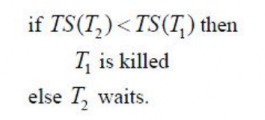
\includegraphics[width=0.4\textwidth]{figures/42.png}
\end{center}
Which of the following is TRUE about the database system using this algorithm?}{42}
\begin{enumerate}
    \item[(A)] Deadlock-free and starvation-free  
    \item[(B)] Deadlock-free but not starvation-free  
    \item[(C)] Starvation-free but not deadlock-free  
    \item[(D)] Neither deadlock-free nor starvation-free  
\end{enumerate}
\vspace{0.5cm}

\questionb{Consider the following grammar:  
}{43}
\begin{center}
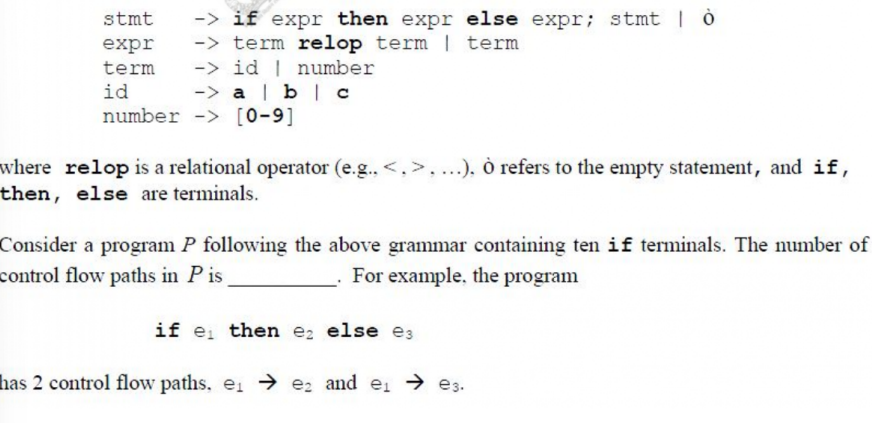
\includegraphics[width=0.9\textwidth]{figures/43.png}
\end{center}
\vspace{0.5cm}

\questionb{In an RSA cryptosystem, a participant \( A \) uses two prime numbers \( p = 13 \) and \( q = 17 \) to generate her public and private keys.  
If the public key of \( A \) is 35, then the private key of \( A \) is \_\_\_\_\_.}{44}
\vspace{0.5cm}

\questionb{The values of parameters for the Stop-and-Wait ARQ protocol are as given below:  
Bit rate = 1 Mbps, propagation delay = 0.75 ms, frame processing time = 0.25 ms,  
information frame = 1980 bytes, acknowledge frame = 20 bytes, overhead per info frame = 20 bytes.  
Assuming no transmission errors, the transmission efficiency (in percentage),  
correct to 2 decimal places, is \_\_\_\_\_.}{45}
\vspace{0.5cm}

\questionb{Consider a database that has the relation schema \texttt{CR(StudentName, CourseName)}.  
An instance of the schema is given below.  
\begin{center}
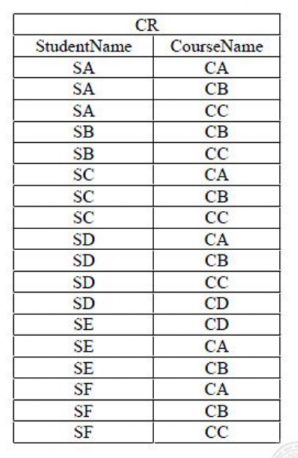
\includegraphics[width=0.3\textwidth]{figures/46.png}
\end{center}
The following query is made on the database:  
\[
T1 \leftarrow \pi_{\text{CourseName}}(\sigma_{\text{StudentName} = 'SA'}(\text{CR})) \\
T2 \leftarrow \text{CR} \div T1
\]  
The number of rows in \( T2 \) is \_\_\_\_\_.}{46}
\vspace{0.5cm}

\questionb{The number of integers between 1 and 500 (both inclusive) that are divisible by 3 or 5 or 7 is \_\_\_\_\_.}{47}
\vspace{0.5cm}

\questionb{Let \( A \) be an array of 31 numbers consisting of a sequence of 0's followed by a sequence of 1's.  
The problem is to find the smallest index \( i \) such that \( A[i] \) is 1 by probing the minimum number of locations in \( A \).  
The worst-case number of probes performed by an optimal algorithm is \_\_\_\_\_.}{48}
\vspace{0.5cm}

\questionb{Consider a RISC machine where each instruction is exactly 4 bytes long.  
Conditional and unconditional branch instructions use PC-relative addressing mode with offset specified in bytes.  
The offset is always with respect to the address of the next instruction.  
Consider the following instruction sequence:  
\begin{center}
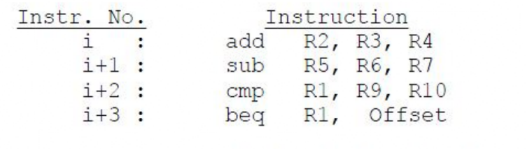
\includegraphics[width=0.5\textwidth]{figures/49.png}
\end{center}
If the target of the branch instruction is instruction \( i \), then the decimal value of the offset is \_\_\_\_\_.}{49}
\vspace{0.5cm}

\questionb{Instruction execution in a processor is divided into 5 stages: Instruction Fetch (IF), Instruction Decode (ID),  
Operand Fetch (OF), Execute (EX), and Write Back (WB). These stages take 5, 4, 20, 10, and 3 ns respectively.  
A pipelined implementation requires 2 ns of buffering delay between each stage.  
Two pipeline implementations are contemplated:\\  
(i) Naive Pipeline (NP): 5 stages \\ 
(ii) Efficient Pipeline (EP): OF stage split into OF1 (12 ns) and OF2 (8 ns)  \\
The speedup (correct to two decimal places) achieved by EP over NP in executing 20 independent instructions with no hazards is \_\_\_\_\_.}{50}
\vspace{0.5cm}

\questionb{Consider a 2-way set associative cache with 256 blocks and LRU replacement policy. Initially, the cache is empty.  
Conflict misses are those misses which occur due to contention of multiple blocks for the same cache set.  
Compulsory misses occur due to first-time access.  
The following sequence of accesses to memory blocks:  
\[
(0,128,256,128,0,128,256,128,1,129,257,129,1,129,257,129)
\]  
is repeated 10 times. The number of conflict misses experienced by the cache is \_\_\_\_\_.}{51}
\vspace{0.5cm}

\questionb{Consider the expression \texttt{(a - 1) * (((b + c) / 3) + d)}.  
Let \( X \) be the minimum number of registers required by an optimal code generation algorithm (no register spills)  
for a load/store architecture where:  
(i) only load and store instructions can access memory  
(ii) arithmetic instructions use only registers/immediates  
The value of \( X \) is \_\_\_\_\_.}{52}
\vspace{0.5cm}

\questionb{Consider the following C program:}{53}
\begin{center}
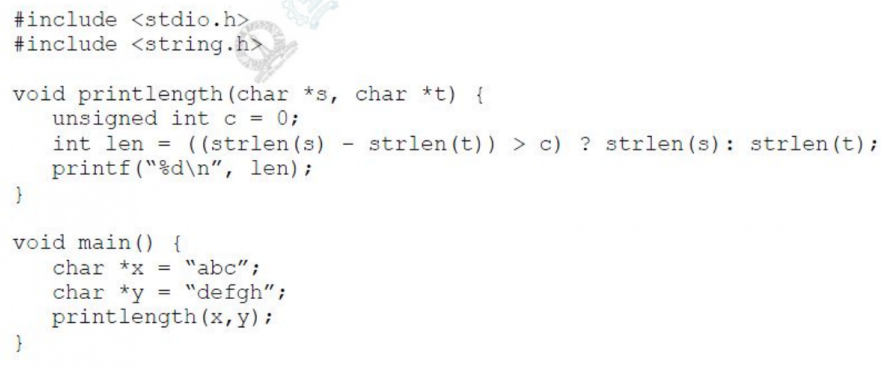
\includegraphics[width=0.9\textwidth]{figures/53.png}
\end{center}
Recall that strlen is defined in string.h as returning a value of type size\_t. which is an
unsigned int. 
 The output of the program is \_\_\_\_\_.  
\vspace{0.5cm}

\questionb{A cache memory unit with capacity of \( N \) words and block size of \( B \) words is to be designed.  
If it is designed as a direct-mapped cache, the length of the TAG field is 10 bits.  
If the cache is now designed as a 16-way set-associative cache, the length of the TAG field is \_\_\_\_\_ bits.}{54}
\vspace{0.5cm}

\questionb{The output of executing the following C program is:}{55}
\begin{center}
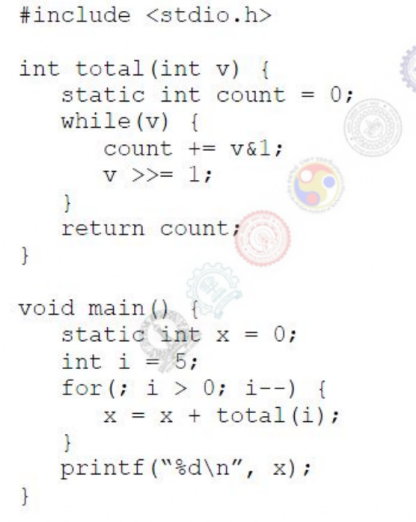
\includegraphics[width=0.3\textwidth]{figures/55.png}
\end{center}
\_\_\_\_\_.  
\vspace{0.5cm}
\vspace{2cm}
\begin{center}
\textbf{END OF THE QUESTION PAPER} \\
\rule{\textwidth}{0.5pt}
\end{center}


\end{document}
